\documentclass[compress, smaller, serif, 9pt]{beamer}


\mode<presentation>
{
  \usetheme{Montpellier}
  %\setbeamercovered{transparent}
  % or whatever (possibly just delete it)
}
% or whatever
%\setbeamertemplate{footline}[frame number]
\beamertemplatenavigationsymbolsempty
\beamertemplatetransparentcovereddynamic

\usepackage[english,frenchb]{babel}
\usepackage[utf8]{inputenc}
% or whatever
%\setbeamertemplate{footline}[frame number]
\beamertemplatenavigationsymbolsempty
\beamertemplatetransparentcovereddynamic
\usefoottemplate{%
       \tinycolouredline{blue!03}%
       {
           \hspace{11.5cm}{\color{black!50} {\insertframenumber $/$ \inserttotalframenumber} \hfill}
       }%
}


% Definitions
%\input{def}
% Raccourcis
%\input{raccourci}

% Beamer settings
%\setbeamercolor{structure}{fg=myem!120}
%\setbeamercolor{example}{bg=LightYell,fg=StroYell}

% \setbeamercolor{alerted text}{fg=lightred}
% \setbeamertemplate{blocks}[rounded][shadow=true]
% \newcommand{\exampletext}[1]{{\usebeamercolor[fg]{example text} #1}}
% \newcommand{\structuretext}[1]{{\usebeamercolor[fg]{structure} #1}}
% \usefonttheme[onlymath]{serif}
% \renewcommand{\thefootnote}{\fnsymbol{footnote}}

%\setbeamerfont{sidebar}{5pt}

\usepackage{amssymb}
%\usepackage[T1]{fontenc}
\usepackage{amsmath,amsthm,bm}
\usepackage{pgf}


\graphicspath{{./Figs/S03/},{./Figs/S02/}}

\usepackage[normal]{subfigure}
\newcommand{\goodgap}{%
    \hspace{\subfigtopskip}%
    \hspace{\subfigbottomskip}}

% les macros
\newcommand{\exampletext}[1]{{\usebeamercolor[fg]{example text} #1}}
\newcommand{\structuretext}[1]{{\usebeamercolor[fg]{structure} #1}}

\newcommand{\bydef}{\stackrel{{def}}{=}}
\newcommand{\ici}{\tcb{$\blacktriangleright \;$}}
\newcommand{\icir}{\alert{$\blacktriangleright \;$}}
\newcommand{\iciex}{\exampletext{$\blacktriangleright \;$}}
\usepackage{pifont}
\newcommand{\doigt}{\structuretext{\noindent \Pisymbol{pzd}{43}}}
\newcommand{\doigtr}{\alert{\noindent \Pisymbol{pzd}{43}}}
\newcommand{\doigtex}{{\exampletext{\noindent \Pisymbol{pzd}{43}}}}

\DeclareMathOperator{\var}{var}
\DeclareMathOperator{\cov}{cov}
\DeclareMathOperator{\trace}{trace}
\DeclareMathOperator{\rank}{rank}
\DeclareMathOperator{\logit}{logit}

\setbeamerfont{block title}{size={\normalsize}}


\title[Statistical Learning]{Machine/Statistical Learning}

\subtitle{Lecture 3: Discriminative approaches\\
Linear regression, Logistic regression}


%\author[Florent Chatelain]{Florent Chatelain}
\institute{Filière SICOM, 3A}
%\logo{\includegraphics[width=.2\textwidth]{logoE3}}
%\date{2015-16}
\date{}

%

\begin{document}

\maketitle

\begin{frame}{Generative vs Discriminative approaches}
 \begin{block}{Generative methods}
 Deduction of $P(Y|X)$ from Bayes rule
 \begin{itemize}
  \item Linear or Quadratic Discriminant Analysis
  \item Naïve Bayes
  \item ...
 \end{itemize}
 \end{block}
 
  \begin{block}{Discriminative methods}
Direct learning of $P(Y|X)$, e.g. generalized linear models s.t.
 \begin{itemize}
  \item Linear regression 
  \item Logistic regression ($\leftarrow$ classification tasks)
  \item ...
 \end{itemize}
 \end{block}
\end{frame}


\section{Linear Regression}

\begin{frame}{Linear Regression Problem}
\begin{minipage}{.48 \textwidth}
\begin{itemize}
 \item $X_i=(X_{i,1}, \ldots, X_{i,p})^T \in \mathbb{R}^p$,
 \item  $Y_i \in \mathbb{R}$, 
\end{itemize}
\end{minipage} \hfill
\begin{minipage}{.5 \textwidth}
 for $i=1,\ldots,n$ (sized $n$ training set)
\end{minipage}

\begin{block}{Linear Regression Model}
\vspace{-5mm}
 \begin{align*}
  Y_i= \beta_0 + \sum_{j=1}^p \beta_j X_{i,j} + \sigma \epsilon_i, \quad \textrm{ for } i=1,\ldots,n, 
 \end{align*}
 \vspace{-5mm}
\begin{itemize}
\item $\epsilon_i$ is a centered with unit variance ($E[ \epsilon_i]= 0$, $\var{(\epsilon_i)}=1$) white noise
\item $\beta_0$ is the ``intercept'' (reduces to the ordinate at the origin when $p=1$)
\item $\structuretext{\beta} \equiv(\beta_{\alert{0}},\ldots,\beta_p) \in \mathbb{R}^{p+\alert{1}}$ is the \structuretext{coefficient vector}
\end{itemize} 
\medskip
\structuretext{Objective:} estimation of $\beta$ $\leftarrow$ supervised learning problem
\end{block}
%\begin{block}{Remark}

\medskip
 \structuretext{Remark:} model linear w.r.t. $\beta$, but not necessarily linear w.r.t.  
 \begin{itemize}
  \item the inputs $X_i$: we can add non linear predictors $h(X_i)$ in the model
  \item the outputs $Y_i$: we can introduce a non linear link function $\leftarrow$ generalized linear model, e.g. logistic regression
 \end{itemize}
%\end{block}

\end{frame}

\begin{frame}{LS (Least Squares) Estimator}

\begin{block}{Definition}
 LS estimate defined by minimizing the Residual Sum of Squares 
\begin{align*}
 \widehat{\beta}&= \arg \min_{\beta} \underbrace{\sum_{i=1}^n \left(y_i- \beta_0 - \sum_{j=1}^p \beta_j x_{i,j} \right)^2}_{\textrm{RSS}(\beta)} 
\end{align*}
\vspace{-3mm}
\begin{itemize}
 \item RSS$(\beta) \ \propto$ empirical error rate for quadratic loss
\end{itemize}

\end{block}


\begin{block}{Matrix expression of RSS}
$$\textrm{RSS}(\beta) = || Y - X \beta ||_2^2,$$
\begin{align*}
\textrm{where }
 Y= \begin{pmatrix} y_1 \\ \vdots \\ y_n \end{pmatrix} \in \mathbb{R}^n, 
 \qquad 
 X= \begin{pmatrix}
     1 & x_{1,1} & \ldots & x_{1,p} \\
     \vdots & \vdots & & \vdots\\
     1 & x_{n,1} & \ldots & x_{n,p} \\
    \end{pmatrix}\in \mathbb{R}^{n\times(p+1)}
\quad
\end{align*}
\end{block}
\end{frame}



\begin{frame}{LS Estimator derivation}


$\widehat{Y}= X \widehat{\beta}$ is the prediction in the space spanned by the column vectors of $X$
such that the euclidean error norm  $|| Y - X \widehat{\beta}||_2$ is minimized

\begin{block}{Orthogonality principle}

Let $X^j$ be the $j$th column of $X$ \medskip \\
\begin{minipage}{.42\textwidth}
\begin{center}
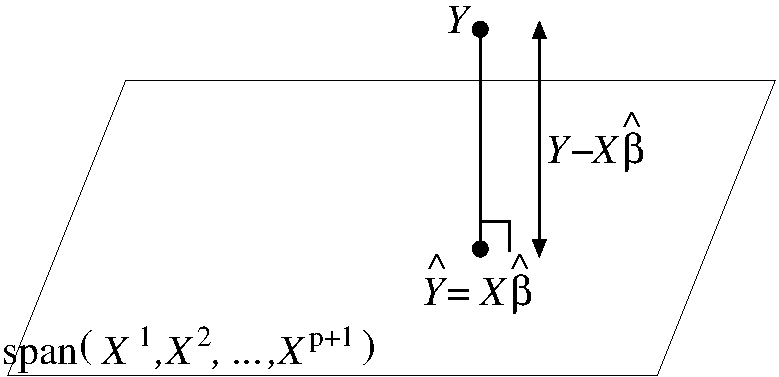
\includegraphics[width=\textwidth]{orthog_principle.pdf}
\end{center}
\end{minipage} \hfill
\begin{minipage}{.55\textwidth}
 for $j=1,\ldots,p+1$
 \begin{align*}
   & \ \langle X^j,Y-X \widehat{\beta} \rangle = (X^j)^T \left(Y- X \widehat{\beta}\right)= 0,\\
   \Leftrightarrow & \quad X^T  \left(Y- X \widehat{\beta}\right)= 0,\\
   \Leftrightarrow  &  \quad\left( X^T X \right)  \widehat{\beta}= X^T Y
 \end{align*}
\end{minipage}

 \end{block}

\end{frame}

\begin{frame}{LS Estimator computation}


Assumption: $\rank{X}=p+1$, hence $ X^T X $ is  invertible%, thus \vspace{-2mm}

\begin{block}{Analytical expression}
\vspace{-5mm}
\begin{align*}
 \structuretext{\widehat{\beta} } &  \structuretext{=\left( X^T X \right)^{-1} X^T Y},
\end{align*}
\vspace{-5mm}
\end{block}

\begin{block}{Numerical computation in high dimension}
When $p>10^{3}$ or $p>10^{4}$, too expansive to compute  $\left( X^T X \right)^{-1}$ ... 
More efficient to use a numerical procedure to minimize the criterion $J(\beta) \equiv\frac{1}{2}\textrm{RSS}(\beta)$, e.g. steepest descent
\begin{align*}
 \beta_{k+1}= \beta_k - \alpha_k \nabla_{\beta} \ J(\beta_k),
\end{align*}
where  step size $\alpha_k \in \mathbb{R}$ is the {\em learning rate}, and descent direction is computed as 
 \begin{itemize}
   \item batch gradient $\nabla_{\beta} \ J(\beta)= X^T X \beta - X^T Y$
   \item stochastic gradient $\nabla_{\beta} \ J(\beta) \approx X_i^T X_i \beta - X_i^T Y_i$ 
   for $i=1,\ldots,n$ (scan of the training set) $\leftarrow$ cheaper than batch one for a single iteration
   \item mini-batch gradient: tradeoff between batch and stochastic gradients
  \end{itemize}
\end{block}
% \end{itemize}
%\end{block}
\end{frame}

\begin{frame}{LS Estimator properties}
For a known $X$, $Y= X \beta + \sigma \varepsilon$ where $E[\varepsilon]=0_n$ and $\cov{\varepsilon}=I_n$.
\begin{itemize}
 \item  $\widehat{\beta}$ is an unbiased estimator of $\beta$
  \begin{align*}
   \structuretext{E[\widehat{\beta}]} &= E \left[ \left( X^T X \right)^{-1} X^T Y \right]= \left( X^T X \right)^{-1} X^T X \beta +  \left( X^T X \right)^{-1} X^T E[\varepsilon] \structuretext{= \beta}
  \end{align*}
\item Covariance \medskip

  $\begin{displaystyle}
   \structuretext{\cov{\widehat{\beta}}}= \left( X^T X \right)^{-1} X^T \cov{(Y)} X \left( X^T X \right)^{-1} 
   %= \left( X^T X \right)^{-1} X^T ( \sigma^2 I_n ) X \left( X^T X \right)^{-1},
   = \structuretext{\sigma^2 \left( X^T X \right)^{-1}}
  \end{displaystyle}$\medskip
\item Power of the estimation error
  \begin{align*}
    \structuretext{E\left[|| \widehat{\beta} - \beta ||^2\right]}&=  E\left[ { \left(\widehat{\beta} - \beta\right)^T \left(\widehat{\beta} - \beta\right) } \right]  
     = E\left[ \trace{ \left(\widehat{\beta} - \beta\right) \left(\widehat{\beta} - \beta\right)^T } \right],\\
    &= \trace{ \left( \cov{\widehat{\beta}} \right) } =  \sigma^2 \trace{\left( \left( X^T X \right)^{-1} \right)}= \structuretext{ \sigma^2 \sum_{j=1}^{p+1} \frac{1}{\lambda_j} }
  \end{align*}
  where  $\lambda_i > 0$ are the eigenvalues of the symm. def. pos. matrix  $X^T X$
 \end{itemize}

 
\end{frame}



\begin{frame}{LS Estimator properties (Cont'd)}
For a known $X$, $Y= X \beta + \sigma \varepsilon$ where $E[\varepsilon]=0_n$ and $\cov{\varepsilon}=I_n$.
\medskip

\begin{block}{Noise variance estimator}
\medskip
An \structuretext{unbiased} estimate of the noise variance $\sigma^2$ can be deduced as
\begin{align*}
  \widehat{\sigma}^2 & = \frac{1}{n \structuretext{-p-1}} \textrm{RSS}\left(\widehat{\beta} \right),
\end{align*}
\end{block}

\begin{block}{Gaussian noise $\varepsilon \sim \mathcal{N}\left(0, I_n\right)$}
\medskip
 \begin{itemize}
  \item $\widehat{\beta}$ is $\mathcal{N}\left(\beta, \sigma^2 \left( X^T X \right)^{-1} \right)$ distributed,
   \item LS estimator $\widehat{\beta}$ is also the maximum likelihood estimator
  \end{itemize}

\end{block}



\end{frame}


\section{Regularization and model selection}

\begin{frame}{Limitations of LS estimator}

\begin{block}{Problem}  
 when $\rank {X} < p+1$, or when $X$ has singular values close to zero, then $ X^T X $ is no more invertible, or 
ill conditioned (eigenvalues close to zero)... 
\end{block}


\begin{block}{Causes} 
\begin{itemize}
 \item redundant or nearly-collinear predictors, e.g. $X^k \approx a X^l + b$, where $X^j$ is the $j$th column of $X$
 \item \alert{high dimensional} problem where \alert{$p \approx n$} (or $p>n$)
\end{itemize}
\end{block}

\begin{block}{Effects} 
no single, or stable, solution for $\widehat{\beta}$
\begin{itemize}
 \item high variance of $\widehat{\beta}$ as an eigenvalue $\lambda_i$ of $X^TX$ is close to zero 
 ($||\widehat{\beta}|| \rightarrow +\infty$ as $\lambda_i \rightarrow 0$),
 \item true error rate  explodes since a small perturbation in the training set  yields a substantially different 
 estimate $\widehat{\beta}$ and prediction rule $\widehat{y}= x^T \widehat{\beta}$ 
 \item[\doigtr] \alert{over-fitting problem} 
\end{itemize}
\end{block}

\end{frame}



\begin{frame}{Regularization}
 

\structuretext{Idea}:  introducing a little bias in the estimation of $\beta$ may lead to
a substantial decrease in variance and, hence, in the true error rate

 
\begin{block}{Penalized regression}
 Regularize the estimation problem by introducing a penalization term for $\beta$
 \begin{align*}
  \widetilde{\beta}= \arg\min_{\beta} \left[ \textrm{RSS}(\beta) + 
  \structuretext{\lambda\, \textrm{Pen}(\beta)}\right]
 \end{align*}
 \vspace{-3mm}
\begin{itemize}
 \item $\textrm{RSS}(\beta)$ is the {\it fidelity term} to the training set,
 \item $\textrm{Pen}(\beta)$ is the {\it a priori} to regularize the solution,
 \item $\lambda > 0$ is the penalization coefficient
\end{itemize}

\end{block}

\hspace{-2.5mm}
\structuretext{Choosing $\lambda$:} tradeoff between overfitting (small $\lambda$) and  underfitting (large $\lambda$)
 \begin{itemize}
  \item[\doigt] standard practice is to use cross-validation to estimate an optimal $\lambda$ for the true 
  error rate (see Lab 1)
 \end{itemize}

\end{frame}

\subsection{Ridge regression}
\begin{frame}{Ridge regression}

Penalization in the (squared) $\ell_2$ sense:
\begin{align*}
 \textrm{Pen}(\beta)&\equiv \beta^T \beta= ||\beta||_2^2, \quad \leftarrow \textrm{Tychonov regularization}
\end{align*}

%\begin{block}{Ridge estimator}
$\widetilde{\beta}$ is thus obtained by minimizing
\begin{align*}
 { \scriptstyle \textrm{RSS}(\beta)    + 
  \lambda\, \textrm{Pen}(\beta)} & { \scriptstyle = 
  (Y-X\beta)^T (Y-X\beta) + \lambda \beta^T \beta,}\\
 & {\scriptstyle = \left( \beta -(X^T X + \lambda I)^{-1} X^T Y \right)^T \left(X^T X + \lambda I\right)
 \left( \beta -(X^T X + \lambda I)^{-1} X^T Y \right) + \textrm{Cst}},
\end{align*}
%Hence, 
\structuretext{Ridge estimator: }
$\begin{displaystyle}
 \widetilde{\beta}= (X^T X + \structuretext{ \lambda I})^{-1} X^T Y
\end{displaystyle}$
\begin{block}{Remark}
  %expression 
  similar to LS estimator,  with an additional 'ridge' on the diagonal of $X^TX$
 \begin{itemize}
  \item $X^T X+\lambda I$ has all its eigenvalues greater than $\lambda > 0$, $\leftarrow$ ensures that
  $\widetilde{\beta}$ is always defined, and stable for large enough $\lambda$
  \item[\doigt] when $\lambda \rightarrow 0$, then $\widetilde{\beta} \rightarrow \widehat{\beta}$,
  \item[\doigt] when $\lambda \rightarrow +\infty$, then  $\widetilde{\beta} \rightarrow 0$
 \end{itemize}

\end{block}
\end{frame}





\begin{frame}
  \frametitle{Ridge Regression: deconvolution illustration}
  \begin{itemize}
   \item $y \in \mathbb{R}^{n}$ with $n=256^2$, \quad $\beta \in \mathbb{R}^{p}$ with $p=256^2$,
   \item $X \in \mathbb{R}^{n \times p} \leftarrow$ sized $(256^2) \times (256^2)$ matrix...
  \end{itemize}

  \begin{overprint}
  \begin{minipage}{.48\textwidth}
  \begin{center}
   
\includegraphics[width=.5\textwidth]{lena_orig.png}\\
   $\beta \leftarrow$ original image
   \end{center}
  \end{minipage} \hfill
  \begin{minipage}{.48\textwidth}
  \begin{center}
   
\includegraphics[width=.5\textwidth]{lena_blurred.png}\\
   $y=X\beta \leftarrow$ blurred image
   \end{center}
  \end{minipage}
  \medskip \\
  \visible<3>{\begin{minipage}{.48\textwidth}
  \begin{center}
   
\includegraphics[width=.5\textwidth]{lena_restored.png}\\
   $\widetilde{\beta} {\scriptstyle	 =  (X^T X+ \lambda I)^{-1} X^T y}\leftarrow$ ridge estimate
   \end{center}
  \end{minipage} \hfill}
  \visible<2,3>{
  \begin{minipage}{.48\textwidth}
  \begin{center}
   
\includegraphics[width=.5\textwidth]{lena_inversed.png}\\
   $\widehat{\beta} {\scriptstyle = (X^T X)^{-1} X^T y} \leftarrow$ LS estimate
   \end{center}
  \end{minipage}}
  \end{overprint}  
\end{frame}


\subsection{Lasso estimator}
\begin{frame}{Regularization by promoting sparsity}

\begin{block}{Sparse representations/approximations}
 A representation, or an approximation, is said to be sparse when most of the coefficients (in a given basis)  are zero
\end{block}


\begin{block}{'Bet on Sparsity' principle}
Sparsity is a good option in high dimension!
 \begin{itemize}
   \item if the sparsity assumption does not hold, no method will be able to recover the underlying model in high dimension where $p\approx n$ or $p>n$
   \item but if the sparsity assumption holds true, then the parameters can be efficiently estimated by
 a method that promotes sparsity
 \item[\doigt] Occam's razor or KISS (keep it simple, stupid) principles: same idea that simpler models are  preferable than more complex ones
 \end{itemize}
\end{block}

\begin{block}{Application to the regression problem}
choosing a penalization function $\textrm{Pen}(\beta)$ that promotes the 
 sparsity of $\beta$ (i.e. with many components $\beta_j=0$ for $j=1,\ldots,p+1$) $\leftarrow$ Lasso estimator
\end{block}

 
\end{frame}



\begin{frame}{Lasso ('least absolute shrinkage and selection operator') estimator}
% 

\begin{block}{Definition} \vspace{-3mm}
  \begin{align*}
  \widetilde{\beta}_{\textrm{lasso}}= \arg\min_{\beta} \left[ \textrm{RSS}(\beta) + 
  \lambda\, \structuretext{||\beta||_1}\right], \vspace{-3mm}
 \end{align*}

 where $||\beta||_1= \sum_{j=1}^{p+1} |\beta_j|$ is the \structuretext{$\ell_1$} norm
\begin{itemize}
 \item no analytical expression of $\widetilde{\beta}_{\textrm{lasso}}$
 \item but convex optimization problem where very efficient numerical procedures are available to compute 
 $\widetilde{\beta}_{\textrm{lasso}}$
 \end{itemize}
\end{block}

\begin{block}{Lasso advantages}
 Converges to a generally \structuretext{sparse} solution, i.e. such that $\beta_k=0$ for a subset of index $k$
 \begin{itemize}
  \item[\doigt] the less significant variables are explicitly discarded
   \item[\doigt] similar stability than ridge estimator + \structuretext{model selection}
 \end{itemize}
\end{block}

\end{frame}





%\section{Penalization with $\ell_1$ and $\ell_2$ norms}

\begin{frame}
  \frametitle{Penalization with $\ell_1$ and $\ell_2$ norms: geometrical interpretation}
  \vspace{-2mm}
{\small
  \begin{itemize}
 \item Least Squares estimator: $\widehat{\beta}= \arg\min \ \textrm{RSS}(\beta)$,
 \item Regularized estimator: $\widetilde{\beta}= \arg\min \left( \textrm{RSS}(\beta) + \lambda \textrm{Pen}(\beta) \right)$ \\
 $\Leftrightarrow$ $\widetilde{\beta}= \arg\min \  \textrm{RSS}(\beta)$ under the constraint 
 $\textrm{Pen}\left(\widetilde{\beta}\right) \le s(\lambda)$.
\end{itemize}
}
\begin{minipage}{.55\textwidth}
\begin{center}
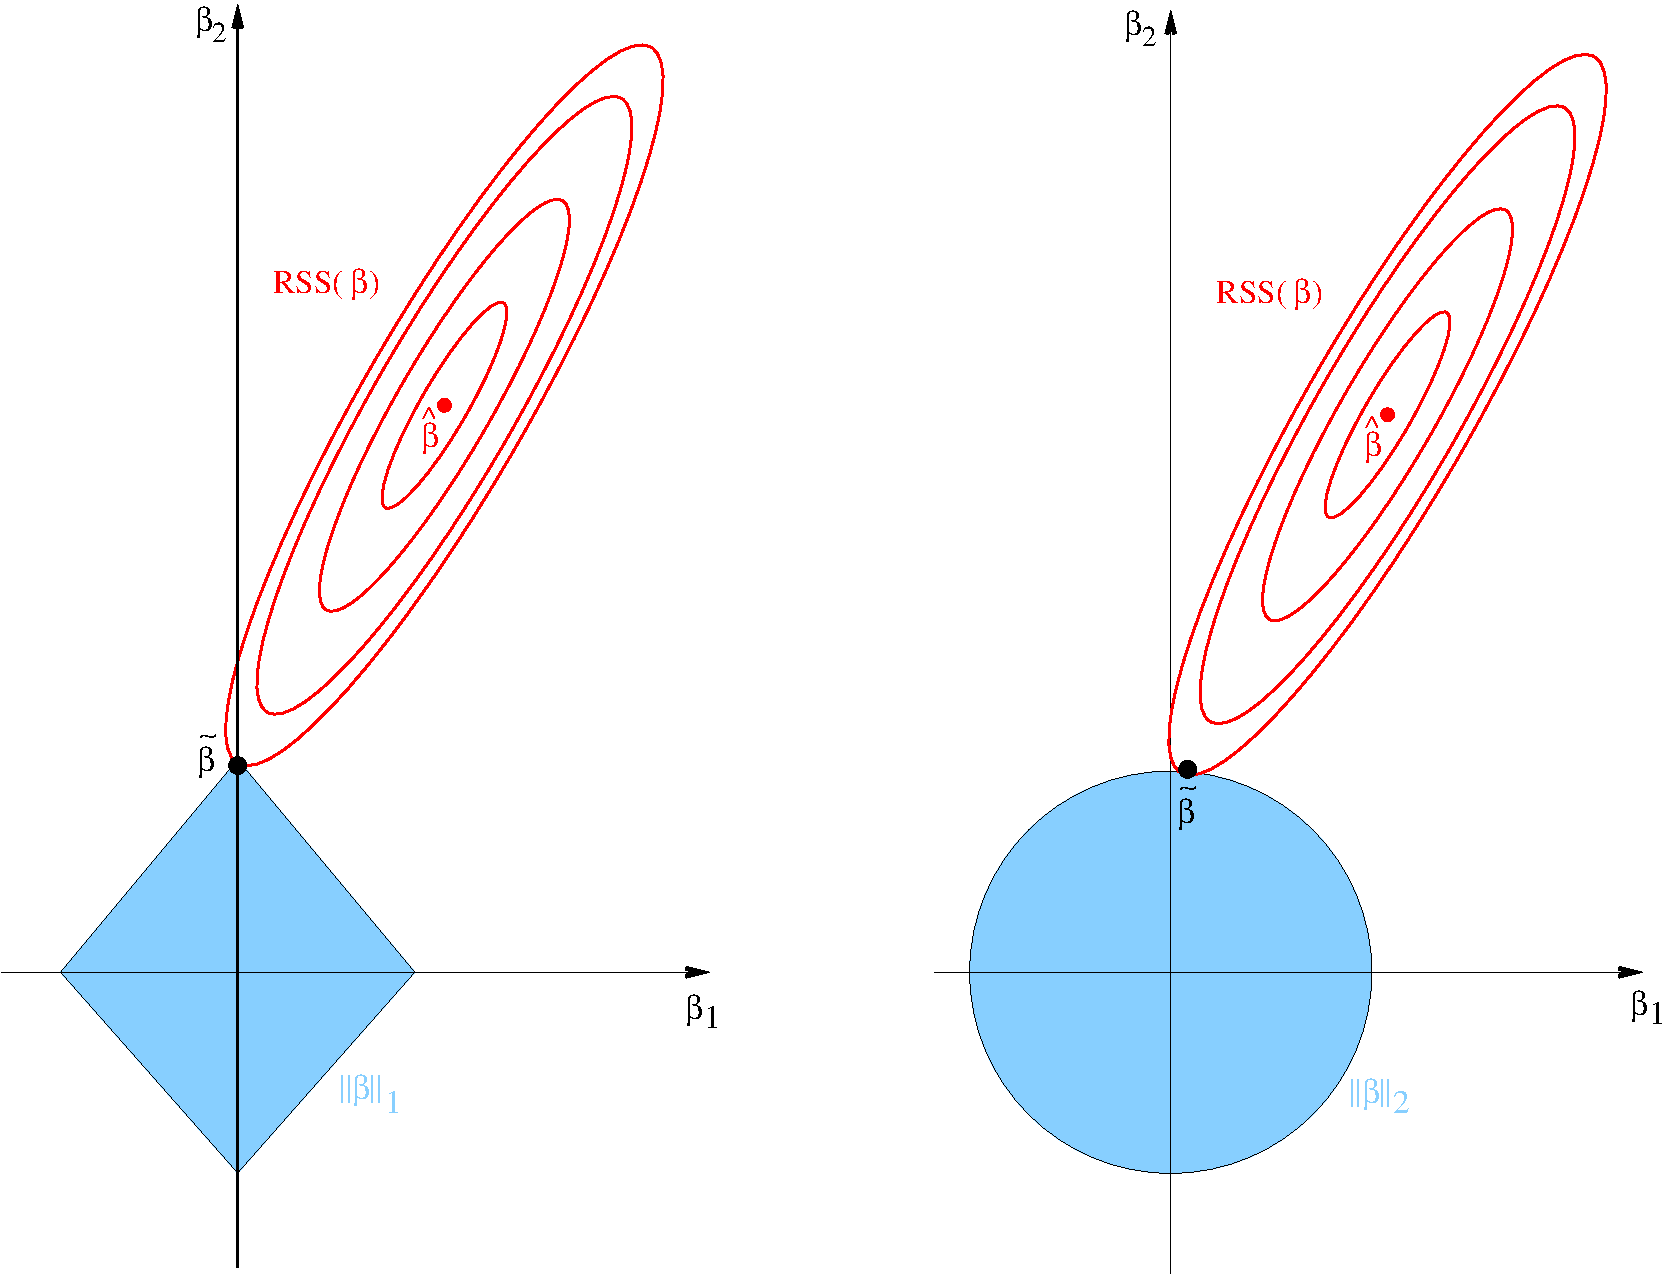
\includegraphics[width=\textwidth]{lasso_geom_ann.pdf}
\end{center}
\end{minipage}
\begin{minipage}{.4\textwidth}
{\small
Illustration in dimension $p=2$~: $\beta=(\beta_1,\beta_2)^T$
\begin{itemize}
\scriptsize
 \item Lasso ($\ell_1$ norm)~: $\textrm{Pen}\left(\beta\right)= ||\beta||_1 = \sum_{k=1}^p |\beta_k|$
 \item Ridge regression ($\ell_2$ squared norm)~: $\textrm{Pen}\left(\beta\right)= ||\beta||_2^2= \beta^T \beta$
\end{itemize}
}
\end{minipage}\\
{\small 
 $\ell_1$ norm promotes the sparsity of the estimator: the less significant predictors are 
 explicitly discarded (coeffs $\beta_k$ are zero)  $\leftarrow$ 
 \textcolor{blue}{model selection}}

\end{frame}


\subsection{Application: prostate data}

\begin{frame}
  \frametitle{Application: prostate data}
 Stamey et al. (1989) study to examine the association between prostate specific antigen (PSA) and several
clinical measures that are potentially associated with PSA in men. Objective is to predict the Log PSA from eight variables  
\begin{itemize}
 \item lcavol: Log cancer volume
 \item lweight: Log prostate weight
  \item age: The man’s age
 \item lbph: Log of the amount of benign hyperplasia
 \item svi: Seminal vesicle invasion; 1=Yes, 0=No
 \item lcp: Log of capsular penetration
 \item gleason: Gleason score
 \item pgg45: Percent of Gleason scores 4 or 5
\end{itemize}
\end{frame}



\begin{frame}
  \frametitle{Application~: prostate data}
\begin{block}{Model selection: $\ell_1$ penalization (Lasso)}
\vspace{-3mm}
$$
\widetilde{\beta}(\lambda) = \arg \min_{\beta} \textrm{RSS}(\beta) + \lambda || \beta ||_{1},
\vspace{-2mm}
$$
$\rightarrow$ function of $\lambda$ where less significant variables are explicitly discarded
%\begin{itemize}
%   \item $\lambda$ petit ($|| \hat{\beta}(\lambda) ||_{1}$ grand) $\rightarrow$ sur-apprentissage
%   \item $\lambda$ grand ($|| \hat{\beta}(\lambda) ||_{1}$ petit) $\rightarrow$ sous-apprentissage
%\end{itemize}
\end{block}
\vspace{-1mm}
\begin{block}{Path of the $\ell_1$-penalized coefficients vs
$|| \widetilde{\beta}(\lambda) ||_{1}$}
\begin{minipage}{.65\textwidth}
\begin{center}
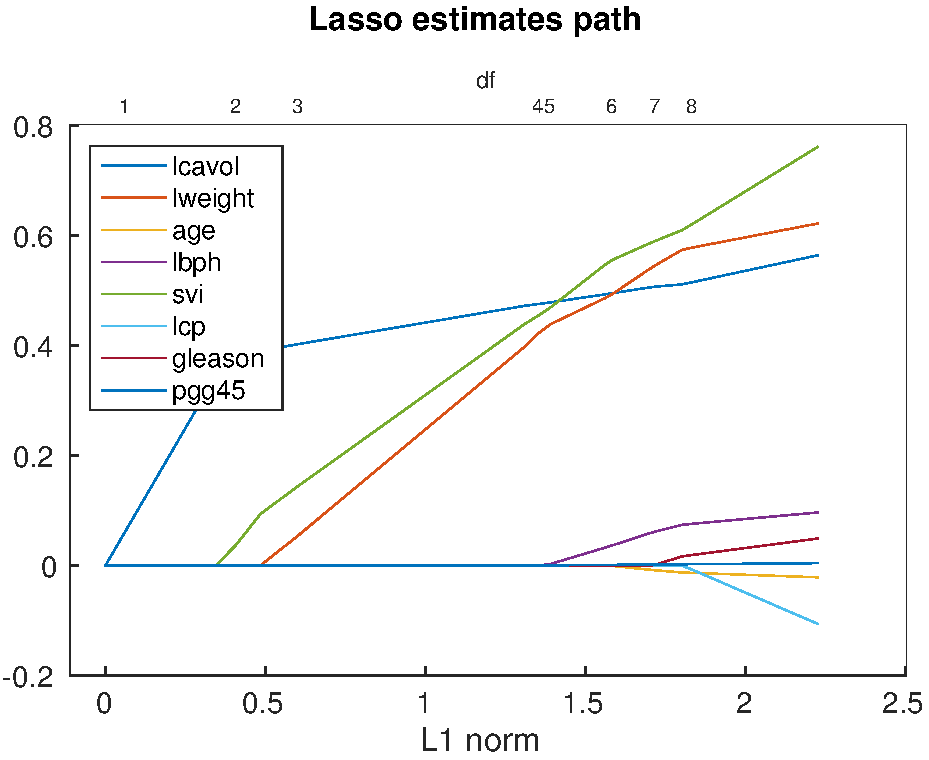
\includegraphics[width=.9\textwidth]{psa_lasso_path.pdf}
\end{center}
\end{minipage}
\begin{minipage}{.33\textwidth}
\small
\textcolor{blue}{Choosing $\lambda$}
\scriptsize
\begin{center}
\begin{itemize}
   \item large  $|| \widetilde{\beta}(\lambda) ||_{1}$  (small $\lambda$)  $\rightarrow$ overfitting
  \item small $|| \widetilde{\beta}(\lambda) ||_{1}$  (large $\lambda$) $\rightarrow$ underfitting
 \item $0.48 \le || \widetilde{\beta}(\lambda) ||_{1} \le 1.43$ $\rightarrow 3$
   predictors (lcavol,svi,lweight)
\end{itemize}
\medskip
$|| \widetilde{\beta}(\lambda) ||_{1}=1.06$ ($\lambda=0.21$) estimated by cross validation
\end{center}
\end{minipage}
\end{block}
\end{frame}

\begin{frame}
  \frametitle{Application~: prostate data}
\begin{block}{Comparison of ridge and lasso  estimators}
\medskip
\begin{minipage}{.48\textwidth}
\begin{center}
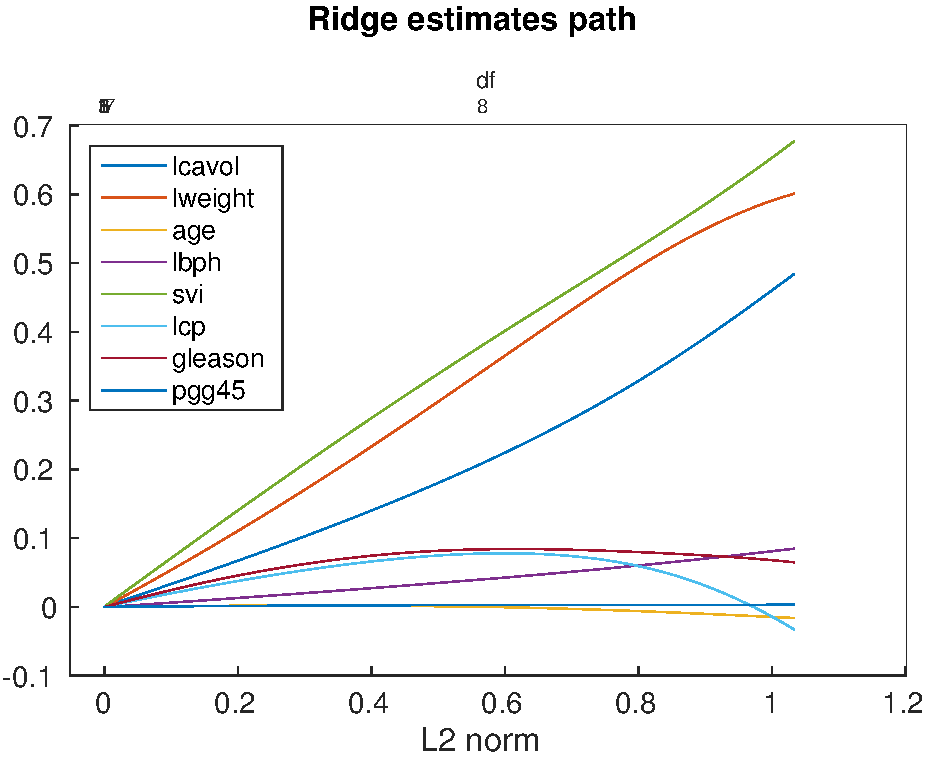
\includegraphics[width=\textwidth]{psa_ridge_path.pdf}
\end{center}
\end{minipage}\hfill
\begin{minipage}{.48\textwidth}
\begin{center}
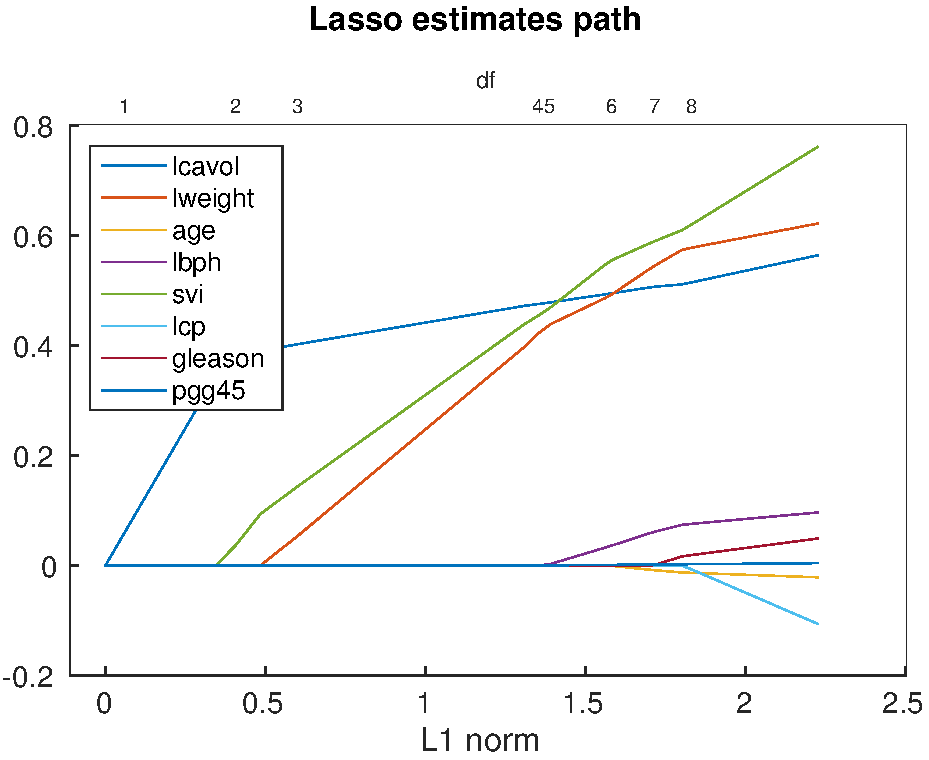
\includegraphics[width=\textwidth]{psa_lasso_path.pdf}
\end{center}
\end{minipage}
 \begin{center}
{Path of the penalized coefficients as a function of
$|| \widetilde{\beta}(\lambda) ||$}  
 \end{center}
\end{block}
\end{frame}

\section{Logistic regression}

\begin{frame}{Logistic regression for binary classification}
 
Classification problem $Y \in \mathcal{Y} \leftarrow$ discrete set
 
 \begin{block}{Binary classification problem: $\mathcal{Y}=\{1,2\}$}
 Consider the following model
 \begin{align*}
  \Pr(Y_i=1 | X_i=x_i) &= \phi(x_i^T \beta)= \frac{\exp{(x_i^T \beta)}}{1+\exp{(x_i^T \beta)}},
 \end{align*}
 where
\begin{itemize}
 \item $x_i=(\structuretext{1},x_{i,1},\ldots,x_{i,p})^T \in \mathbb{R}^{p+\structuretext{1}}$ $\leftarrow$  
 \structuretext{intercept} term included by default,
 \item $\structuretext{\phi}: \ u \in \mathbb{R} \mapsto \frac{\exp{(u)}}{1+\exp{(u)}} \in (0,1)$ is the \structuretext{logistic} function: maps  a real value to  a probability
 \end{itemize}



 \end{block}

\end{frame}



\begin{frame}
  \frametitle{Logistic function}
\begin{align*}
   \phi(x)~: \mathbb{R} &\rightarrow \, ]0,1[\\
                u &\mapsto \frac{\exp{u}}{1 + \exp{u}} = \frac{1}{1 + \exp{(-u)}}.
\end{align*}


\begin{center}
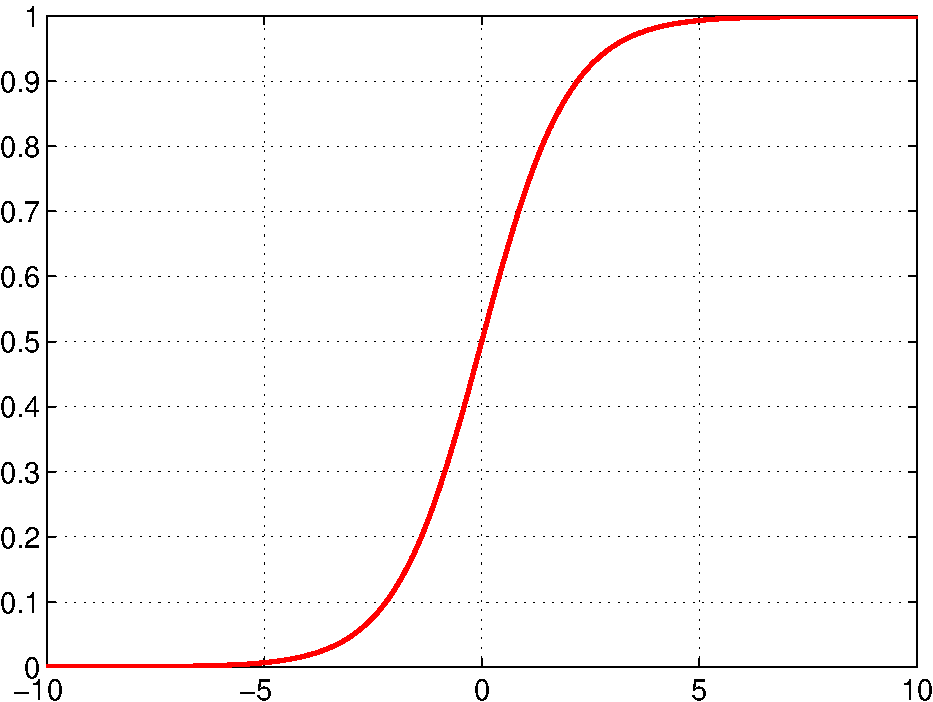
\includegraphics[width=.6\textwidth]{logisitc_func.pdf}
\end{center}
\end{frame}




\begin{frame}{Logit link function}
 
Consider   
 \begin{itemize}
   \item $p_i \equiv \Pr(Y_i=1 | X_i=x_i) = \phi(x_i^T \beta)$
 \item $\structuretext{\phi^{-1}}: \ p \in (0,1) \mapsto \log \frac{p}{1-p} \in \mathbb{R}$ is the \structuretext{logit} function
\end{itemize}

\begin{block}{Generalized linear model }
\begin{itemize}
 \item  \structuretext{Linear} equation  w.r.t. $\beta$, 
 \begin{align*}
         \logit{(p_i)}= x_i^T \beta, 
        \end{align*}
 \item  additional \structuretext{nonlinear} constraint:
 \begin{align*} \Pr(Y_i=2 | X_i=x_i) = 1-\underbrace{\Pr(Y_i=1| X_i=x_i)}_{p_i}=  \frac{1}{1+\exp{(x_i^T \beta)}}\end{align*}
\end{itemize}


\end{block}

\end{frame}


\begin{frame}{Logistic regression for classification in $K$ classes}
 
% Classification problem in $Y \in \mathcal{Y} \leftarrow$ discrete set
 When $\mathcal{Y}=\{1,\ldots,K\}$ $\leftarrow$ $K$ classes,  the models becomes
 
 %\begin{block}{General case:  $\mathcal{Y}=\{1,\ldots,K\}$}
$$
 \begin{array}{lcl}
 \log \frac{\Pr(Y_i=1 | X_i=x_i)}{\Pr(Y_i=K | X_i=x_i)} &=& x_i^T \beta_1,\\
 \log \frac{\Pr(Y_i=2 | X_i=x_i)}{\Pr(Y_i=K | X_i=x_i)} &=& x_i^T \beta_2,\\
 \hspace{15mm} \vdots & & \quad \vdots\\
 \log \frac{\Pr(Y_i=K-1 | X_i=x_i)}{\Pr(Y_i=K | X_i=x_i)} &=& x_i^T \beta_{K-1},
 \end{array}$$
\begin{itemize}
 \item[\doigt] $K-1$ equations +  sum-to-one constraint on the probabilities
\end{itemize}

\medskip
\begin{block}{General case: logistic equations}
\vspace{-3mm}
\begin{align*}
\Pr(Y_i=\structuretext{k} | X_i=x_i) &=  \frac{\exp{(x_i^T \beta_\structuretext{k})}}{1+ \sum_{l=1}^{K-1} \exp{(x_i^T \beta_l)}}, \quad \textrm{ for } k=1,\ldots,K-1,\\
 \Pr(Y_i=\structuretext{K} | X_i=x_i) &=  \frac{1}{1+\sum_{l=1}^{K-1} \exp{(x_i^T \beta_l)}}
  \end{align*}
\end{block}


\end{frame}

\begin{frame}{Parameter estimation}
 Since the distribution of $Y|X$ is known, the log-likelihood expresses as \vspace{-2mm}
 \begin{align*}
  \ell(\beta)&= \sum_{i=1}^n \log{ p_{X,Y}(x_i,y_i|\beta)},\\
  &=  \sum_{i=1}^n \log{ p_{Y|X}(y_i|x_i,\beta)} + \sum_{i=1}^n \log{ p(x_i)}, \quad \leftarrow \textrm{Bayes rule}\vspace{-2mm}
 \end{align*}
 where the second term is a constant that does not depend on $\beta$
 
 
 \medskip
 \begin{block}{Maximum likelihood estimator}
 \medskip
 Maximizing the log-likelihood w.r.t $\beta$ $\Leftrightarrow$ Maximizing the conditional log-likelihood  
 $\beta \mapsto \sum_{i=1}^n \log{ p_{Y|X}(y_i|x_i,\beta)}$
\begin{itemize}
 \item no analytical expression of the ML estimator,
 \item numerical computation performed by a Newton-Raphson procedure, which reduces to an 
 iterative reweighted least squares (IRLS) algorithm
 \item Rk: regularized estimator defined as $\widetilde{\beta} = \arg \min_{\beta} -\ell(\beta) + \lambda \textrm{Pen}(\beta)$
\end{itemize}
\end{block}

\end{frame}

\begin{frame}{ML estimator computation}

\begin{block}{Newton-Raphson's method for binomial ($K=2$) logistic regression}
 Iterative procedure to converge to the root of the score function $\frac{ \partial \ell(\beta) }{ \partial \beta }$, \vspace{-2mm}
 \begin{align*}
  \beta_{\textrm{new}} \leftarrow \beta_{\textrm{old}} - \left( \frac{ \partial^2 \ell(\beta) }{ \partial \beta \partial \beta^T } \right)^{-1} \frac{\partial\ell(\beta)}{\partial \beta},\vspace{-3mm}
 \end{align*} 
 Assuming that $y\in \mathcal{Y}=\{0,1\}$, then
  \begin{align*}
   \ell(\beta) &= \sum_{i=1}^n y_i \log \phi(x_i^T \beta) + (1-y_i) \log \left(1 - \phi(x_i^T \beta) \right)+\textrm{Cst}.
  \end{align*}
 It comes that $\frac{\partial\ell(\beta)}{\partial \beta}  =  X^T (y-p)$, and 
  $ \frac{ \partial^2 \ell(\beta) }{ \partial \beta \partial \beta^T } =  X^T W X,$ where
 \begin{itemize}
  \item $X \equiv$ $n\times(p+1)$ matrix with $i$th line $x_i^T$ (including the intercept coefficient)
  \item $p \equiv$ sized $n$ vector of probability with $i$th element $\phi(x_i^T \beta)$,
  \item $W\equiv$  $n\times n$ diagonal matrix with $i$th diagonal element $\phi(x_i^T \beta)  \left(1-\phi(x_i^T \beta) \right)$
 \end{itemize}
 \end{block}
 

\end{frame}


\begin{frame}{ML estimator computation (Cont'd)}
 \begin{block}{Newton-Raphson's algorithm for binomial ($K=2$) logistic regression} \medskip
Repeat until convergence\\
$\left\lfloor \begin{array}{rcl}
 Z&=& X  \beta_{\textrm{old}} + W^{-1} (Y-p),\\
\beta_{\textrm{new}}&\leftarrow &\arg \min_{\beta} \left(Z-X\beta\right)^T W \left(Z-X\beta\right)= \left(X^TWX\right)^{-1} W Z
\end{array} \right.$ \medskip \\
where $W$ and $p$ are evaluated for $\beta= \beta_{\textrm{old}}$

\end{block}

\begin{itemize}  
 \item[\doigt] iterative reweighted least squares (IRLS) procedure with a nonlinear in $\beta$ weight matrix $W$
 \item[\doigt] can be extended to the multiclass case ($K\ge 3$) with a $(K-1)n\times(K-1)n$  nondiagonal weight matrix $W$ composed of $(K-1)^2$ diagonal $n\times n$ submatrices (fast implementations are available)
 \item[\doigt] regularized estimator computation: gradient descent like methods can be used
\end{itemize}
 
\end{frame}



\section{Application: heart diseases data}

\begin{frame}
  \frametitle{Application:  South African coronary heart disease (CHD)}
\begin{minipage}{.55\textwidth}
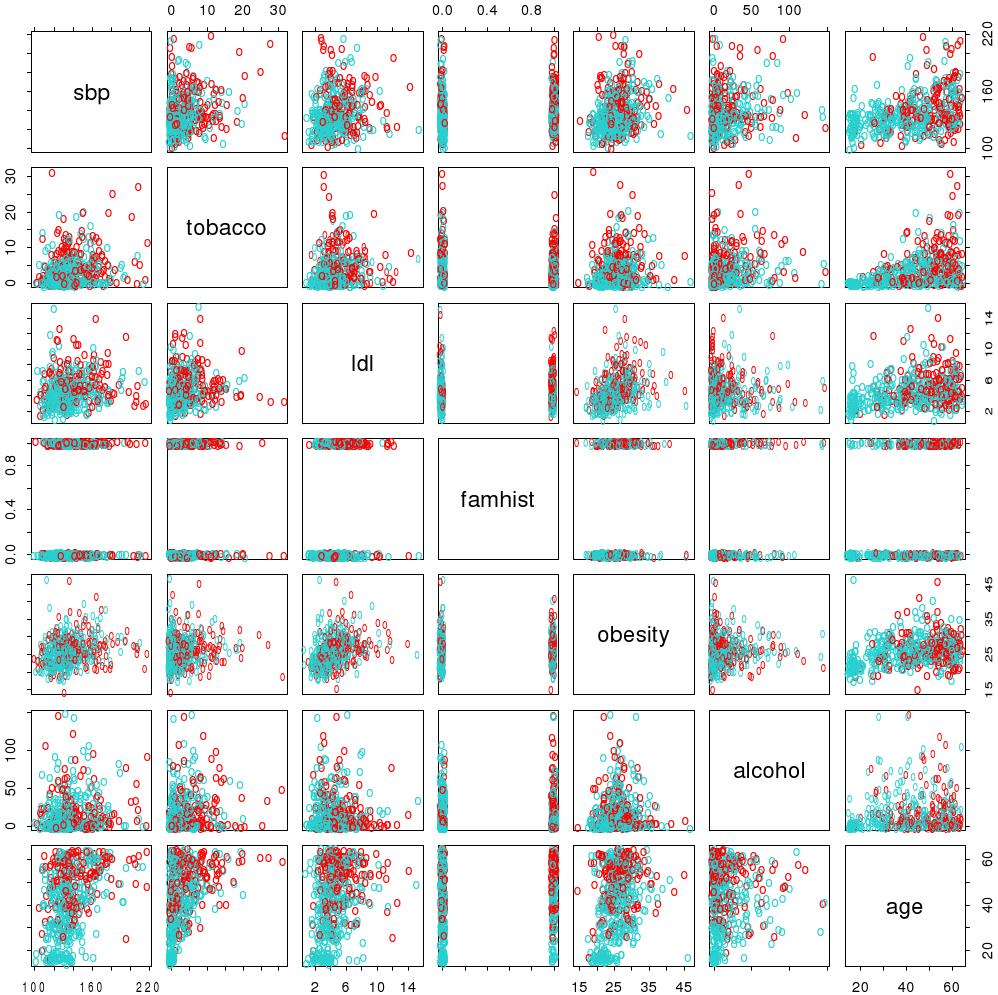
\includegraphics[width=\textwidth]{heartdiseases_scatter.jpg}
\end{minipage}
\hfill
\begin{minipage}{.4\textwidth}
\begin{block}{Matrix of the predictor scatterplots}
\end{block}
\begin{itemize}
   \item each plot $\equiv$ pair of risk factors
   \item $160$ \textcolor{red}{cases} / $302$ \textcolor{cyan}{controls}
   \item {\it ldl}: $\sim$ cholesterol,  {\it sbp}: systolic blood pressure
\end{itemize}
\end{minipage}

\end{frame}

\begin{frame}
  \frametitle{Application: South African CHD (Cont'd)}

\begin{block}{Logistic regression fit}
\begin{center}
\small
\begin{tabular}{rrrr}\hline
& Coefficient & Std. Error & $Z$ score\\
\hline
\texttt{(Intercept)} & $-4.130$ & $0.964$ & $-4.285$\\
\texttt{sbp} & $0.006$ & $0.006$ & $1.023$\\
\texttt{tobacco} & $0.080$ & $0.026$ & $3.034$\\
\texttt{ldl} & $0.185$ & $0.057$ & $3.219$\\
\texttt{famhist} & $0.939$ & $0.225$ & $4.178$\\
\texttt{obesity} & $-0.035$ & $0.029$ & -$1.187$\\
\texttt{alcohol} & $0.001$ & $0.004$ & $0.136$\\
\texttt{age} & $0.043$ & $0.010$ & $4.184$\\
\hline
\end{tabular} 
\end{center}
%\begin{center}
%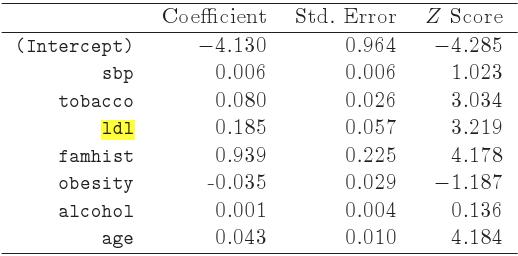
\includegraphics[width=.65\textwidth]{table_logreg_heartdiseases.jpg}
%\end{center}
\end{block}
\begin{itemize}
   \item A  $Z$ score ( $\equiv$ Coeff / Std. Error)  $> 2$ in absolute value is  significant at
   the $5$\% level.
\end{itemize}
\begin{alertblock}{Must be interpreted with caution!}
\begin{itemize}
   \item systolic blood pressure (sbp) is not significant! 
   \item nor is obesity (conversely, $<0$ coefficient)!
   \item[$\rightarrow$] result of the strong correlations between the predictors
\end{itemize}
\end{alertblock}
\end{frame}


\begin{frame}
  \frametitle{Application: South African CHD (Cont'd)}

\begin{block}{Model selection}
Find the variables that are sufficient for explaining the CHD outputs\\
\begin{itemize}
   \item drop the least significant predictor, and refit the model
   \item repeat until no further terms can be dropped  $\leftarrow$ \structuretext{backward selection}
\end{itemize}
\end{block}
\vspace{-2mm}
\begin{block}{Logistic regression fit with backward model selection procedure}
\begin{center}
\small
\begin{tabular}{rrrr}\hline
& Coefficient & Std. Error & $Z$ score\\
\hline
\texttt{(Intercept)} & $-4.204$ & $0.498$ & $-8.45$\\
\texttt{tobacco} & $0.081$ & $0.026$ & $3.16$\\
\texttt{ldl} & $0.168$ & $0.054$ & $3.09$\\
\texttt{famhist} & $0.924$ & $0.223$ & $4.14$\\
\texttt{age} & $0.044$ & $0.010$ & $4.52$\\
\hline
\end{tabular} 
\end{center}
%\begin{center}
%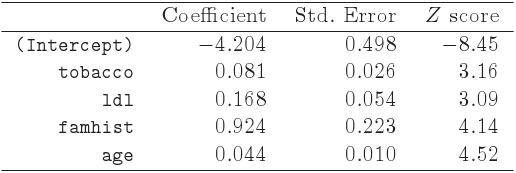
\includegraphics[width=.65\textwidth]{table_logreg_heartdiseases_red.jpg}
%\end{center}
\end{block}
\vspace{-6mm}
\begin{block}{Interpretations}
\begin{itemize}
   \item Tobacco is measured in total lifetime usage in kilograms, with a median of 1kg
   for the controls and 4.1kg for the cases
   \item An increase of  1kg $\Rightarrow$ increase of the CHD proba of 
    $\exp{(0.081)}=1.084$ or $8.4$\% (confidence interval at $95$\% $[1.03,1.14]$)
\end{itemize}
\end{block}
\end{frame}



\begin{frame}
  \frametitle{Application:  South African CHD (Cont'd)}
\begin{block}{Model selection: $\ell_1$ penalization (Lasso type method)}
\vspace{-3mm}
$$
\widetilde{\beta}(\lambda) = \arg \min_{\beta} - \ell(\beta) + \lambda || \beta ||_{1},
\vspace{-2mm}
$$
$\rightarrow$ function of $\lambda$ where less significant variables are explicitly discarded
%\begin{itemize}
%   \item $\lambda$ petit ($|| \hat{\beta}(\lambda) ||_{1}$ grand) $\rightarrow$ sur-apprentissage
%   \item $\lambda$ grand ($|| \hat{\beta}(\lambda) ||_{1}$ petit) $\rightarrow$ sous-apprentissage
%\end{itemize}
\end{block}
\vspace{-1mm}
\begin{block}{Path of the  des coefficients $\ell_1$-penalized coefficients as a function of
$|| \hat{\beta}(\lambda) ||_{1}$}
\begin{minipage}{.65\textwidth}
\begin{center}
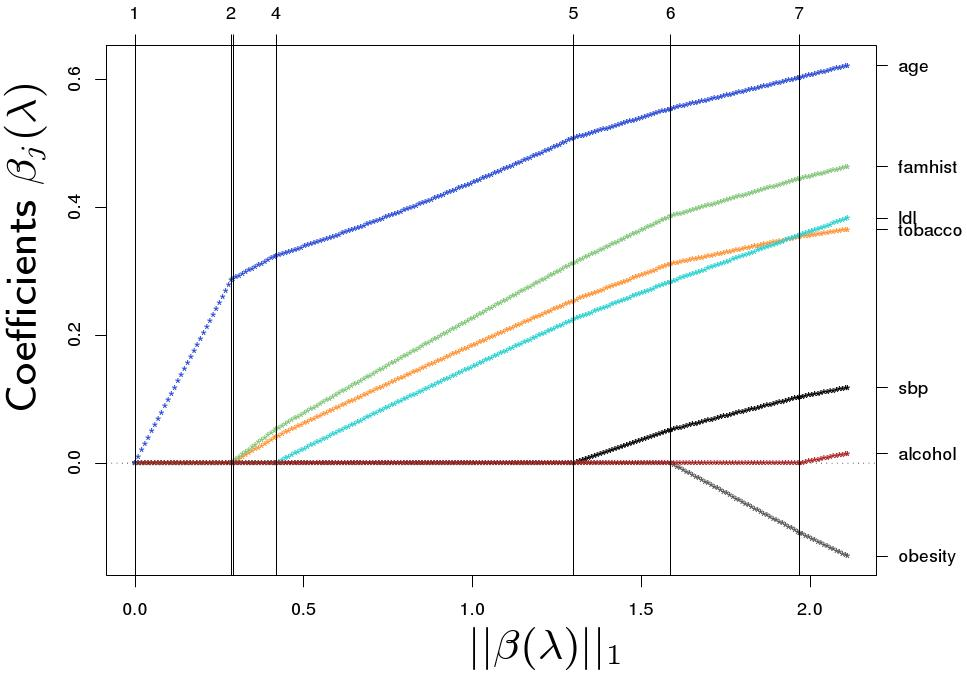
\includegraphics[width=\textwidth]{path_lasso_heartdiseases.jpg}
\end{center}
\end{minipage}
\begin{minipage}{.33\textwidth}
\small
\textcolor{blue}{Choosing $\lambda$}
\scriptsize
\begin{center}
\begin{itemize}
   \item large $|| \widetilde{\beta}(\lambda) ||_{1}$ (small $\lambda$)  $\rightarrow$ overfitting
  \item small $|| \widetilde{\beta}(\lambda) ||_{1}$ (large $\lambda$) $\rightarrow$ underfitting
 \item $0.43 \le || \widetilde{\beta}(\lambda) ||_{1} \le 1.3$ $\rightarrow 4$
   same predictors than backward selection procedure
\end{itemize}

\end{center}
\end{minipage}
\end{block}
\end{frame}


\section{Linear Discriminant Analysis vs Logistic Regression}

\begin{frame}{Linear Discriminant Analysis vs Logistic Regression}

Example for binary classification problem $\mathcal{Y}=\{1,2\}$
\begin{block}{Linear Discriminant Analysis (LDA)}
\vspace{-3mm}
\begin{align*}
\log \frac{\Pr(Y=2 | X=x)}{\Pr(Y=1 | X=x)} &= \alpha_0 + x^T \alpha, 
\end{align*}\vspace{-3mm}
\begin{itemize}
 \item $\begin{displaystyle}
         \alpha_0= \log \frac{\pi_2}{\pi_1} - \frac{1}{2} (\mu_1+  \mu_2) \Sigma^{-1}(\mu_2 -  \mu_1),    
        \end{displaystyle}$
 \item $\begin{displaystyle} \alpha=  \Sigma^{-1} (\mu_2 -  \mu_1) \end{displaystyle}$
\end{itemize}

\end{block}

\begin{block}{Logistic regression}\vspace{-5mm}
\begin{align*}
\log \frac{\Pr(Y=2 | X=x)}{\Pr(Y=1 | X=x)} &= \beta_0 + x^T \beta, 
\end{align*}
\end{block}

\begin{itemize}
 \item both models give classification rules linear w.r.t. $x$,
 \item Logistic regression is not based on a Gaussian assumption and can be more robust on real-word data
\end{itemize}


\end{frame}


\begin{frame}
  \frametitle{Example}
\begin{block}{Mixture of $K=3$ Gaussians}
\begin{itemize}
   \item $Y \in \{\textcolor{red}{1},\textcolor{green}{2},\textcolor{blue}{3}\}$
   \item $X \in \mathbb{R}^2$
\end{itemize}
\end{block}
\vspace*{-8mm}

\begin{center}
  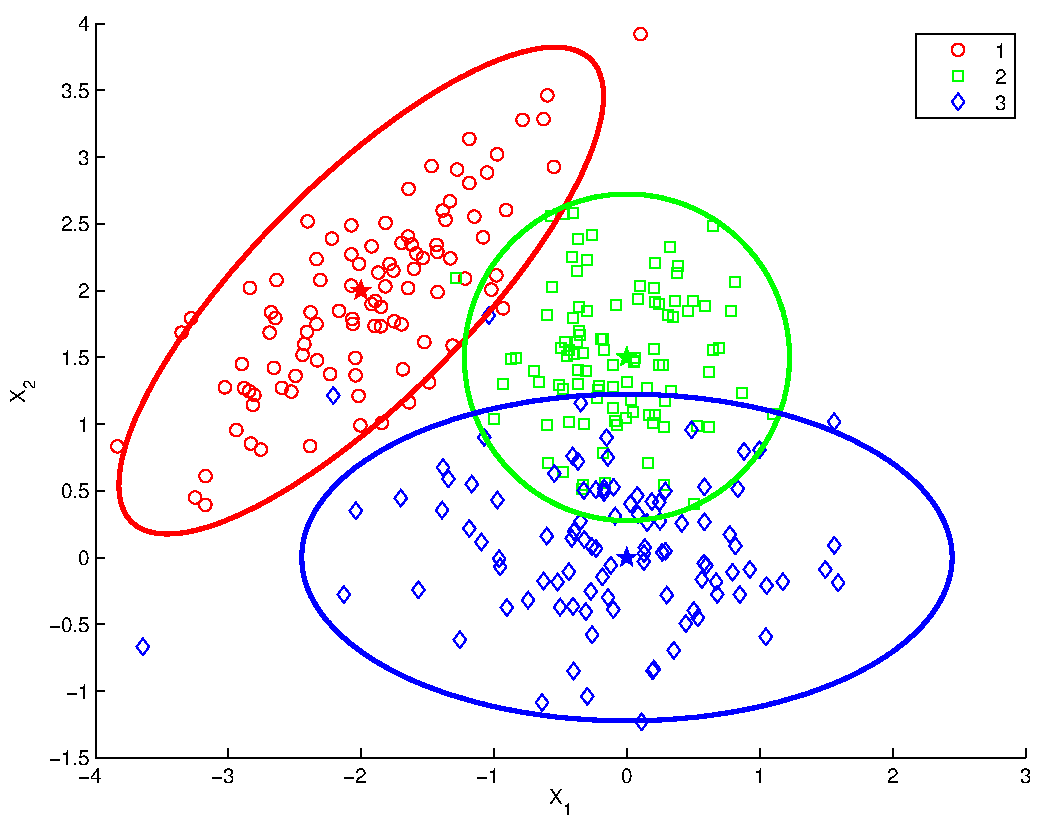
\includegraphics[width=.65\textwidth]{discr_analysis_CI.pdf} \\
  True confidence regions at $95\%$ level
\end{center}

\end{frame}



\begin{frame}
  \frametitle{Linear Discriminant Analysis (LDA)}
\begin{block}{Mixture of $K=3$ Gaussians}
\begin{itemize}
   \item  Classification rule $\arg \max_{k=\textcolor{red}{1},\textcolor{green}{2},\textcolor{blue}{3}}
\delta_k(x)$
\item linear boundaries  $\{ x ; \delta_k(x)=\delta_l(x) \} $
\end{itemize}
\end{block}
\vspace*{-4mm}

\begin{center}
  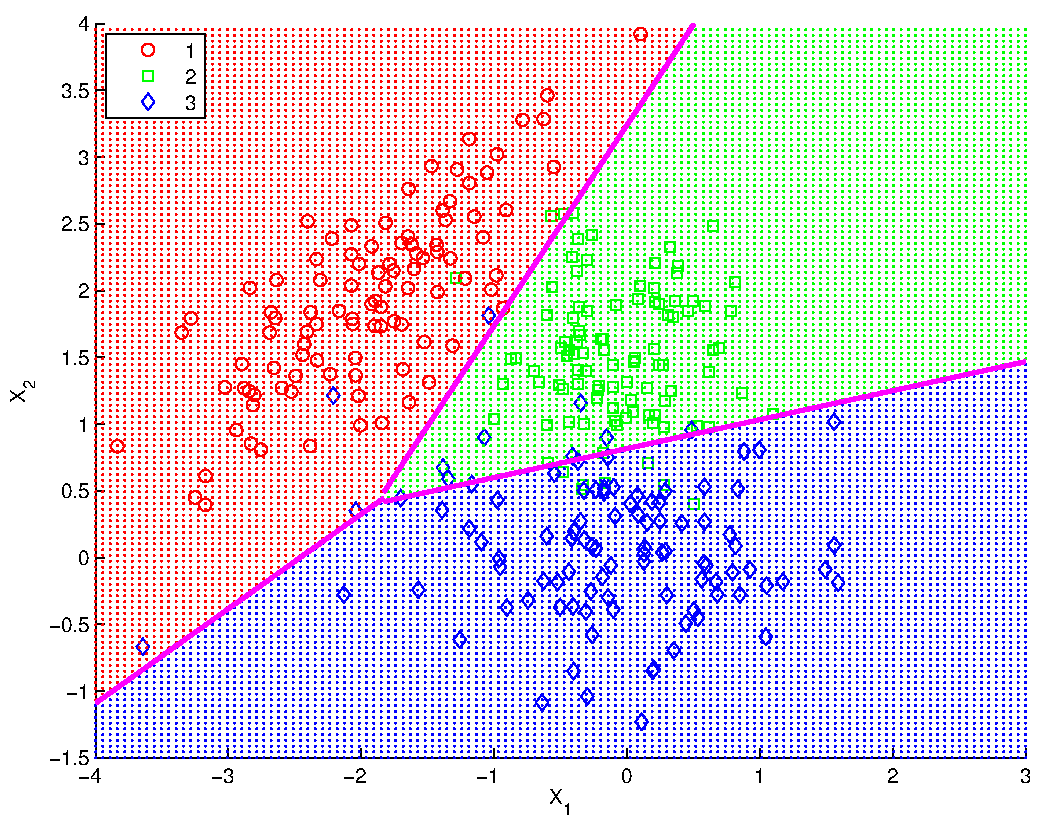
\includegraphics[width=.65\textwidth]{linear_analysis_bounds.pdf} \\
\end{center}

\end{frame}

\begin{frame}
  \frametitle{Logistic regression}
\begin{block}{Mixture of $K=3$ Gaussians}
\begin{itemize}
   \item   Classification rule $\arg \max_{k=\textcolor{red}{1},\textcolor{green}{2},\textcolor{blue}{3}}
\pi_k(x)$
\item linear boundaries  $\{ x ; \log{ \frac{p_k(x)}{p_l(x)} } = 0 \} $
\end{itemize}
\end{block}
\vspace*{-4mm}

\begin{center}
  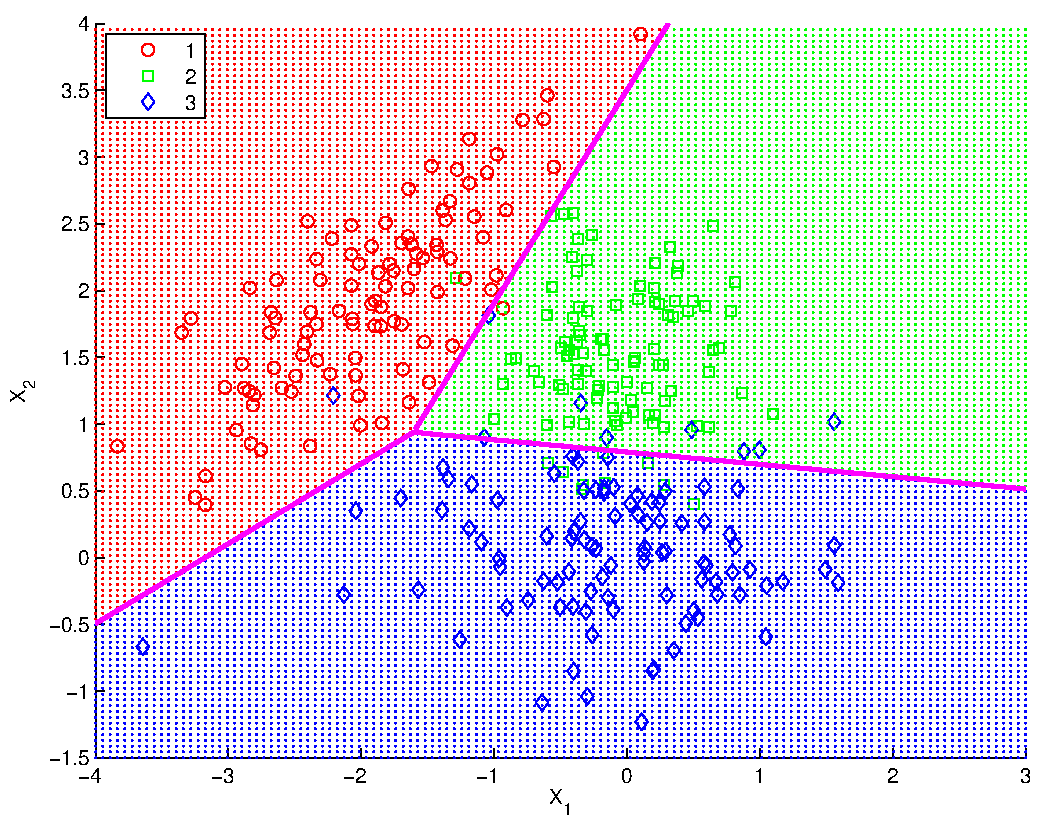
\includegraphics[width=.65\textwidth]{log_analysis_bounds.pdf} \\
\end{center}

\end{frame}

\begin{frame}
  \frametitle{Conclusions}
  \begin{block}{Discriminative Approaches}
   Learning  of the prediction rule based on a model of $Y$ given $X$
   \begin{itemize}
    \item[\doigt] Linear regression, Logistic regression
   \end{itemize}
  \end{block}
  
  \begin{block}{Perspectives}
  'Black box' methods (model free) to learn the  prediction rule 
   \begin{itemize}
    \item[\doigt] (Deep) Neural nets, SVM
   \end{itemize}

  \end{block}

\end{frame}

\end{document}
